\documentclass{article}
\usepackage{iclr2026_conference,times}

\usepackage{amsmath}
\usepackage{amssymb}
\usepackage{amsfonts}
\usepackage{amsthm}
\usepackage{algorithm}
\usepackage{algorithmic}
\usepackage{graphicx}
\usepackage{booktabs}
\usepackage{multirow}
\usepackage{xcolor}
\usepackage{hyperref}
\usepackage{url}
\usepackage{tikz}
\usetikzlibrary{shapes.geometric,arrows.meta,positioning,fit,backgrounds,calc}

\newtheorem{theorem}{Theorem}
\newtheorem{proposition}[theorem]{Proposition}
\newtheorem{assumption}{Assumption}
\newtheorem{definition}{Definition}

% Visible marker for projected results. Delete this macro definition and every use
% of it once the Stage-1 experiments have been executed and real numbers substituted.
\newcommand{\projected}{\textcolor{red}{\textbf{[PROJECTED]}}}

\title{When the Safety Signal Lies:\\Adversarial Corruption of Safety-Cost\\Feedback in Constrained Multi-Agent RL}

\author{Anonymous}

\begin{document}

\maketitle

\begin{abstract}
Safe multi-agent reinforcement learning (MARL) assumes the safety-cost signal used to enforce constraints is reported faithfully. In decentralized deployments this is unwarranted: primal-dual methods exchange \emph{learned} cost estimates and Lagrange multipliers over a network, making the constraint-enforcement channel itself attackable. We formalize the constrained Markov game with corrupted cost feedback and show this threat is structurally distinct from reward poisoning rather than a relabeling of it. Our central result is a \emph{corruption mass conservation} property: because consensus mixing matrices are doubly stochastic, the aggregate dual-variable bias injected by corrupted reports is invariant to network topology, connectivity, and spectral gap. Consensus cannot dilute cost corruption; it redistributes a concentrated attack on one agent into a diffuse attack on all $N$ agents, each perturbed below any per-agent detection threshold. We further show dual bias enters the policy gradient multiplicatively, scaled by the constraint-gradient norm, amplifying the attack precisely at the constraint boundary. We then give a defense, Robust Constraint Estimation (RCE), combining trimmed-mean aggregation with an uncertainty margin and a bounded multiplier; we prove bounded constraint violation whenever fewer than half the reporting sources are corrupted, and liveness under over-reporting attacks that defeat update-gating defenses. \textbf{The empirical results in Section~\ref{sec:exp} are projected implementation targets, not measured outcomes; they are marked throughout and require validation before this work is submitted as an empirical claim.}
\end{abstract}

\section{Introduction}
\label{sec:intro}

Reinforcement learning agents deployed in safety-critical settings -- multi-robot coordination, power-grid control, autonomous driving fleets -- must respect explicit safety constraints, not merely maximize return. Constrained Markov decision processes (CMDPs) formalize this for a single agent \citep{altman1999cmdp}, and constrained policy optimization \citep{achiam2017cpo,tessler2019rcpo,chow2018lyapunov,stooke2020pid} extends policy search to the constrained setting with near-constraint-satisfaction guarantees. Multi-agent extensions include MACPO and MAPPO-Lagrangian \citep{gu2023macpo}, decentralized primal-dual actor-critic methods \citep{lu2021decentralized,ying2024scalable,kahe2024distributed}, and standardized benchmarks \citep{ji2023safetygym,ray2019benchmarking} built atop MAPPO \citep{yu2022mappo} and PPO \citep{schulman2017ppo}.

This literature shares a standing assumption: the safety-cost signal $C$ used to enforce the constraint is observed correctly, or corrupted only by benign estimation noise. In a decentralized deployment this is not obviously true. Decentralized primal-dual methods require agents to exchange locally estimated costs and Lagrange multipliers over a communication network, and as work on distributed constrained MARL notes explicitly, these exchanged quantities are \emph{learned variables} rather than raw environment observations, so networking them enlarges the attack surface \citep{kahe2024distributed}. A shared or learned cost critic is likewise software that can be compromised, misconfigured, or -- in the case of a malicious teammate -- deliberately dishonest.

An immediate objection is that this is reward poisoning \citep{zhang2020adaptive,rakhsha2020policyteaching,wang2024rlhfpoison} with the letter $r$ replaced by the letter $C$. In a CMDP, reward and cost are both scalar signals entering a scalar objective, so the substitution looks notational. \textbf{The central technical claim of this paper is that it is not.} The cost signal does not enter the policy update the way reward does: it drives a dual variable, that dual variable multiplies the entire constraint gradient, and in decentralized methods it is consensus-averaged across the network. These three facts compose into a threat with properties reward poisoning does not have, and Section~\ref{sec:theory} makes them precise.

Specifically, we prove that the aggregate dual bias produced by corrupted cost reports is \emph{independent of the mixing matrix} (Theorem~\ref{thm:mass}). Doubly stochastic consensus preserves the total injected corruption exactly, no matter how well connected the network is. What consensus changes is not the magnitude but the distribution: a persistent attack by a single agent asymptotically biases \emph{every} agent's multiplier by $\eta_\lambda\delta K/N$ rather than biasing one agent's by $\eta_\lambda\delta K$. For safety this is strictly worse. A violation by any one agent is a system-level failure, so spreading the same corruption mass across $N$ agents converts one conspicuously miscalibrated agent into $N$ agents each miscalibrated below a per-agent detection threshold. Stealth is not incidental to this attack; it is a structural consequence of the consensus step that decentralized safe MARL relies on.

\textbf{Contributions.}
\begin{itemize}
\item We formalize the constrained Markov game with corrupted cost feedback (Section~\ref{sec:formulation}): the full game tuple, an explicit adversary model with knowledge and budget assumptions, and a corruption taxonomy organized along four orthogonal axes rather than as a flat list.
\item We establish that cost corruption is structurally distinct from reward corruption (Section~\ref{sec:theory}): corruption mass is conserved under consensus regardless of topology (Theorem~\ref{thm:mass}), and dual bias enters the policy gradient multiplicatively, amplified by $\|\nabla_\theta J_C\|$ near the constraint boundary (Proposition~\ref{prop:mult}).
\item We give Robust Constraint Estimation (RCE) (Section~\ref{sec:defense}), prove a bounded-violation guarantee under $M \ge 2f+1$ (Theorem~\ref{thm:bounded}), and prove liveness under over-reporting (Proposition~\ref{prop:liveness}) -- a failure mode that defeats the natural update-gating defense.
\item We specify a complete evaluation protocol and report projected implementation targets (Section~\ref{sec:exp}), including a breakdown study exhibiting the predicted failure at $2f \ge M$.
\end{itemize}

\textbf{Status of the empirical claims.} The results in Sections~\ref{sec:theory} and~\ref{sec:defense} are proved in Appendix~\ref{app:proofs}. The numbers in Section~\ref{sec:exp} are \emph{projected implementation targets} derived from methodological analysis, marked \projected{} at every occurrence: design specifications against which we will validate an implementation, not measured results, and not to be read as evidence. Section~\ref{sec:limitations} states what this does and does not license us to claim.

\section{Related Work}
\label{sec:related}

\textbf{Safe RL and constrained MDPs.} The CMDP formalism \citep{altman1999cmdp} separates a task objective from safety costs under a budget. CPO \citep{achiam2017cpo} gave the first general-purpose trust-region method with per-iteration near-constraint-satisfaction guarantees; RCPO \citep{tessler2019rcpo}, Lyapunov-based methods \citep{chow2018lyapunov}, and PID control of the multiplier \citep{stooke2020pid} are the main alternatives, surveyed by \citet{gu2024reviewsaferl} and situated within trustworthy RL by \citet{xu2022trustworthy}. PID-Lagrangian is directly relevant here: by changing how cost error propagates into the multiplier it alters the attack's transfer function, so we treat it as a baseline rather than an afterthought.

\textbf{Safe MARL.} MACPO and MAPPO-Lagrangian \citep{gu2023macpo} were the first safe MARL algorithms with monotonic-improvement and constraint-satisfaction guarantees. A parallel line develops \emph{decentralized} primal-dual algorithms that replace a central trainer with local updates plus consensus on the dual variables \citep{lu2021decentralized,ying2024scalable,kahe2024distributed}, building on classical distributed optimization \citep{nedic2009distributed}. Safety-Gymnasium \citep{ji2023safetygym} and Safety Gym \citep{ray2019benchmarking} provide standardized benchmarks. This literature already recognizes that the quantities exchanged in decentralized safe MARL are learned rather than observed, and that exchanging them is an exposure \citep{kahe2024distributed}; we ask what happens when that exposure is exploited, and show that the consensus step is what makes the exploitation stealthy.

\textbf{Byzantine and adversarial robustness in MARL.} \citet{li2024byzantine} formalize Byzantine cooperative MARL as a Bayesian game in which any agent may act arbitrarily. Others harden MARL via minimax objectives \citep{li2019robust}, model-uncertainty-aware training \citep{zhang2020robustmodel}, evolutionary auxiliary attackers \citep{yuan2023robust}, adversarial value decomposition \citep{phan2021resilient}, and adversarial regularization \citep{bukharin2024robust}; single-agent analogues include \citet{pinto2017robust}, \citet{tessler2019action}, and certified robustness to observation perturbation \citep{zhang2020robustdeep,huang2017adversarial}. These target \emph{actions} or \emph{observations}; none models the cost report as an adversarial channel.

\textbf{Poisoning, backdoors, and corruption-robust theory.} Reward poisoning perturbs $r_t \to r_t + \delta_t$ to steer an agent toward a target policy, with adaptive \citep{zhang2020adaptive} and environment-poisoning \citep{rakhsha2020policyteaching} variants; RLHFPoison \citep{wang2024rlhfpoison} corrupts preference data. Backdoor attacks on RL \citep{kiourti2020trojdrl} and competitive MARL \citep{wang2021backdoorl} implant trigger-conditioned behavior and are the closest existing analogue to our selective-corruption axis. Adversarial policies \citep{gleave2020adversarial} manipulate a victim through physically realizable actions alone. Corruption-robust RL theory bounds regret under an adversarial budget on reward or transition observations \citep{lykouris2024corruption,ye2024towards}. Our defense borrows aggregation primitives from Byzantine-robust distributed learning -- trimmed mean and coordinate-wise median \citep{yin2018byzantine} and Krum \citep{blanchard2017krum} -- and we make that debt explicit rather than presenting them as new. Separately, a non-adversarial literature reaches our thesis from the opposite direction: when the measured signal diverges from the intended one, optimization exploits the gap \citep{amodei2016concrete,skalse2022defining}. Corrupted cost feedback is the adversarial instance of that phenomenon, and Section~\ref{sec:exp} includes a benign-critic-error control to separate the two.

\textbf{Positioning.} Table~\ref{tab:positioning} places our threat model against the closest alternatives. The claim is narrow: not that Byzantine or safe MARL are new, but that manipulating the specific signal used to enforce a constraint has distinct structure -- established in Section~\ref{sec:theory} -- that no existing threat model captures.

\begin{table}[t]
\caption{Positioning relative to the closest threat models. The distinguishing property of cost corruption is that the corrupted signal drives a \emph{dual} variable which is consensus-averaged and which multiplies the constraint gradient; this is what produces Theorem~\ref{thm:mass}.}
\label{tab:positioning}
\centering
\footnotesize
\begin{tabular}{@{}llll@{}}
\toprule
\textbf{Threat model} & \textbf{Channel attacked} & \textbf{Enters update via} & \textbf{Work} \\
\midrule
Reward poisoning & Task reward $r_t$ & Objective, additively & \citep{zhang2020adaptive} \\
Backdoor / Trojan RL & Observation trigger & Policy network & \citep{kiourti2020trojdrl} \\
Adversarial policy & Victim observations & Environment dynamics & \citep{gleave2020adversarial} \\
Byzantine MARL & Compromised actions & Joint action & \citep{li2024byzantine} \\
\textbf{Cost corruption (ours)} & \textbf{Safety cost $C^i_t$} & \textbf{Dual var., multiplic.} & \textbf{--} \\
\bottomrule
\end{tabular}
\end{table}

\section{Constrained Markov Games with Corrupted Cost Feedback}
\label{sec:formulation}

\subsection{The Game}

\begin{definition}[Constrained Markov game]
\label{def:cmg}
A constrained Markov game is a tuple $\mathcal{M} = \langle \mathcal{N}, \mathcal{S}, \{\mathcal{A}^i\}, P, R, \{C^i\}, \{d^i\}, \gamma, \rho_0 \rangle$ where $\mathcal{N} = \{1,\dots,N\}$ is a set of agents, $\mathcal{S}$ a state space, $\mathcal{A}^i$ agent $i$'s action space with joint space $\mathcal{A} = \prod_i \mathcal{A}^i$, $P : \mathcal{S}\times\mathcal{A}\to\Delta(\mathcal{S})$ a transition kernel, $R : \mathcal{S}\times\mathcal{A}\to\mathbb{R}$ a shared task reward, $C^i : \mathcal{S}\times\mathcal{A}\to\mathbb{R}_{\ge 0}$ a per-agent safety cost with budget $d^i$, $\gamma\in(0,1)$ a discount factor, and $\rho_0$ an initial state distribution.
\end{definition}

For a joint policy $\pi_\theta = \prod_i \pi^i_{\theta^i}$ define the task return and the per-agent cost return
\begin{equation}
J_R(\theta) = \mathbb{E}_{\pi_\theta}\Big[\textstyle\sum_{t\ge 0}\gamma^t R(s_t,a_t)\Big],
\qquad
J_C^i(\theta) = \mathbb{E}_{\pi_\theta}\Big[\textstyle\sum_{t\ge 0}\gamma^t C^i(s_t,a_t)\Big].
\label{eq:returns}
\end{equation}
The cooperative constrained objective is to find $\theta^\star \in \arg\max_\theta J_R(\theta)$ subject to $J_C^i(\theta)\le d^i$ for all $i\in\mathcal{N}$. We adopt per-agent constraints because they are the setting of the decentralized primal-dual methods we attack \citep{lu2021decentralized,ying2024scalable,kahe2024distributed}; the shared-constraint case $\frac{1}{N}\sum_i J_C^i \le d$ is recovered by taking $W = \frac{1}{N}\mathbf{1}\mathbf{1}^\top$ in Section~\ref{sec:theory}. We distinguish the \emph{per-step} cost $C^i_t \triangleq C^i(s_t,a_t)$ from the \emph{return} $J^i_C$: the budget $d^i$ constrains the return, and every constraint we write is on the return scale, since the defense in Section~\ref{sec:defense} operates on return-scale estimates throughout.

\subsection{Learner and Adversary}

We consider the standard decentralized primal-dual learner \citep{lu2021decentralized,kahe2024distributed}. Each agent $i$ holds policy parameters $\theta^i$ and a multiplier $\lambda^i \ge 0$, and maintains a local cost critic producing an estimate $\hat{J}^i_C$ of its cost return. Agents communicate over a connected graph $\mathcal{G}$ with doubly stochastic mixing matrix $W$ (so $W\mathbf{1}=\mathbf{1}$ and $\mathbf{1}^\top W = \mathbf{1}^\top$), and run
\begin{equation}
\theta^i_{k+1} = \theta^i_k + \eta_\theta \nabla_{\theta^i}\big[J_R(\theta_k) - \lambda^i_k J^i_C(\theta_k)\big],
\qquad
\lambda_{k+1} = \Pi_{[0,\lambda_{\max}]}\big[W\lambda_k + \eta_\lambda\, g_k\big],
\label{eq:primaldual}
\end{equation}
where $\lambda_k = (\lambda^1_k,\dots,\lambda^N_k)^\top$ and $g^i_k = \hat{J}^i_C(\theta_k) - d^i$ is the local constraint residual. The projection onto $[0,\lambda_{\max}]$ is standard and keeps the multiplier bounded.

\begin{definition}[Corrupted cost feedback]
\label{def:corruption}
An adversary controls a set $\mathcal{B}\subset\mathcal{N}$ of at most $f = |\mathcal{B}|$ reporting sources. For $i\in\mathcal{B}$ the residual entering Eq.~\eqref{eq:primaldual} is replaced by $\tilde{g}^i_k = g^i_k + \delta^i_k$; equivalently, at the per-step level agent $i$ reports $\tilde{C}^i_t = C^i_t + \delta^i_t$. For $i\notin\mathcal{B}$ we have $\tilde{g}^i_k = g^i_k$. We write $\delta_k\in\mathbb{R}^N$ for the stacked corruption vector, supported on $\mathcal{B}$.
\end{definition}

\textbf{Adversary knowledge and capability.} We assume the adversary (i)~observes the reports and multipliers traversing the channels it controls, (ii)~may choose $\delta_k$ as a function of the learner's current iterate $(\theta_k,\lambda_k)$, giving an adaptive attack, (iii)~cannot modify rewards, actions, observations, or transitions, and (iv)~is subject to a per-round budget $\|\delta_k\|_\infty \le B$ and, where stated, a cumulative budget $\sum_k\|\delta_k\|_1 \le \Delta$, following the corruption-budget framing of \citet{lykouris2024corruption} and \citet{ye2024towards}. Restriction~(iii) makes the threat model non-trivial rather than artificial: it corresponds to a deployment whose control plane is authenticated but whose telemetry plane is not, the common configuration in fielded multi-robot and industrial-control systems. Section~\ref{sec:limitations} revisits its realism.

\subsection{Corruption Taxonomy}

Informal lists of attack types mix incomparable notions. We organize corruption along four orthogonal axes, so an attack is a point in a product space rather than a row in a list (Table~\ref{tab:taxonomy}). This matters operationally: the axes are independently controllable, whereas a flat list produces overlapping conditions that cannot be varied one at a time.

\begin{table}[t]
\caption{Corruption taxonomy as four orthogonal axes. An attack instance selects one value per axis; for example, the primary attack studied in Section~\ref{sec:exp} is (negative, persistent, static, consistent), and the stealth attack is (negative, selective, adaptive, consistent).}
\label{tab:taxonomy}
\centering
\small
\begin{tabular}{@{}llp{6.4cm}@{}}
\toprule
\textbf{Axis} & \textbf{Values} & \textbf{Interpretation} \\
\midrule
Direction & negative / positive / mixed & Sign of $\delta^i_k$: under-reporting hides violations; over-reporting induces over-conservatism or denial of learning. \\
Support & persistent / selective & Whether all rounds are corrupted or only a strategically chosen subset, trading attack strength against detectability. \\
Adaptivity & static / adaptive & Whether $\delta_k$ is fixed or is a function of $(\theta_k,\lambda_k)$. \\
Consistency & consistent / Byzantine & Whether a source reports the same value to all peers or equivocates across peers and rounds. \\
\bottomrule
\end{tabular}
\end{table}

\textbf{The mechanism of concern.} Corrupted reports bias the dual variable, the biased multiplier distorts the constrained policy update, and the resulting policy violates the true constraint -- while the reported cost, being the corrupted quantity, continues to look acceptable. The attack matters exactly when task reward stays high, because reward and reported cost are the only two quantities standard evaluation observes. Figure~\ref{fig:pipeline} draws the two paths this divergence requires, and Section~\ref{sec:theory} shows why the divergence is not merely possible but structurally favored.

\begin{figure}[t]
\centering
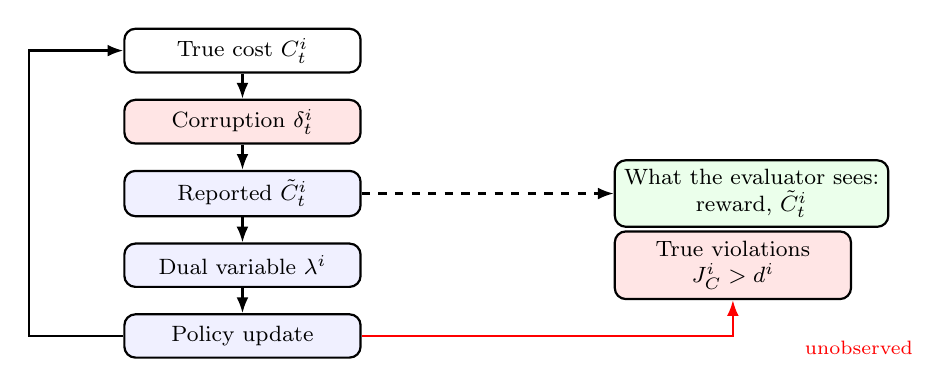
\begin{tikzpicture}[
  node distance=3.2mm and 14mm,
  n/.style={draw, rounded corners, thick, minimum height=5.5mm, minimum width=30mm, align=center, font=\footnotesize},
  bad/.style={draw, rounded corners, thick, minimum height=5.5mm, minimum width=30mm, align=center, font=\footnotesize, fill=red!10},
  ok/.style={draw, rounded corners, thick, minimum height=5.5mm, minimum width=30mm, align=center, font=\footnotesize, fill=blue!6},
  arr/.style={-{Latex[length=2mm]}, thick}
]
\node[n] (true) {True cost $C^i_t$};
\node[bad, below=of true] (corrupt) {Corruption $\delta^i_t$};
\node[ok, below=of corrupt] (report) {Reported $\tilde C^i_t$};
\node[ok, below=of report] (dual) {Dual variable $\lambda^i$};
\node[ok, below=of dual] (policy) {Policy update};
\node[bad, right=32mm of dual] (violation) {True violations\\$J^i_C > d^i$};
\node[n, right=32mm of report, fill=green!8] (monitor) {What the evaluator sees:\\reward, $\tilde C^i_t$};

\draw[arr] (true) -- (corrupt);
\draw[arr] (corrupt) -- (report);
\draw[arr] (report) -- (dual);
\draw[arr] (dual) -- (policy);
\draw[arr] (policy.west) -- ++(-12mm,0) |- (true.west);
\draw[arr, red, thick] (policy.east) -| (violation.south);
\draw[arr, dashed] (report.east) -- (monitor.west);
\node[font=\scriptsize, red] at ($(violation.south)+(16mm,-6mm)$) {unobserved};
\end{tikzpicture}
\caption{Corrupted safety-feedback pipeline. The learner closes its loop entirely through the reported path (left column), and the evaluator observes only task reward and the reported cost (green). True violations (red) are caused by the resulting policy but are never fed back, which is what permits reported and true safety to diverge without any visible symptom.}
\label{fig:pipeline}
\end{figure}

\section{Cost Corruption Is Not Reward Corruption}
\label{sec:theory}

This section substantiates the paper's central claim. We isolate the effect of corruption on the dual trajectory, show that consensus conserves it exactly (Theorem~\ref{thm:mass}), characterize how it spreads (Corollary~\ref{cor:spread}), and show that it reaches the policy gradient multiplicatively rather than additively (Proposition~\ref{prop:mult}). Proofs are in Appendix~\ref{app:proofs}.

Let $\lambda_k$ denote the dual trajectory under corruption and $\lambda^\circ_k$ the trajectory of the same algorithm, from the same initialization and along the same primal sequence, under uncorrupted reports. Define the \emph{dual bias} $e_k \triangleq \lambda_k - \lambda^\circ_k$. Throughout this section we assume both trajectories remain in the interior of $[0,\lambda_{\max}]$, so the projection in Eq.~\eqref{eq:primaldual} is inactive; Appendix~\ref{app:proofs} discusses the projected case, where the conclusions hold with inequality rather than equality.

\begin{theorem}[Corruption mass conservation]
\label{thm:mass}
Under the decentralized primal-dual update of Eq.~\eqref{eq:primaldual} with any doubly stochastic mixing matrix $W$, the dual bias satisfies $e_K = \eta_\lambda\sum_{k=0}^{K-1} W^{K-1-k}\delta_k$, and its aggregate obeys
\begin{equation}
\mathbf{1}^\top e_K \;=\; \eta_\lambda \sum_{k=0}^{K-1}\mathbf{1}^\top\delta_k .
\label{eq:mass}
\end{equation}
The right-hand side does not depend on $W$. Hence the total dual bias across the network is invariant to the communication topology, its connectivity, and its spectral gap.
\end{theorem}

This inverts a common intuition. Consensus averaging is normally stabilizing -- it is what makes decentralized optimization converge to the centralized solution -- and one might expect averaging over many honest reports to attenuate a single dishonest one. Equation~\eqref{eq:mass} says it does not attenuate it at all: double stochasticity is exactly the property that preserves the sum, so the structure that makes consensus work is the structure that makes it unable to reject corruption mass. Connectivity, extra communication rounds, and a larger spectral gap change only how fast the bias equilibrates, never how much there is.

\begin{proposition}[Spreading]
\label{cor:spread}
Let a single corrupted agent $j$ inject a persistent bias $\delta_k = \delta e_j$ for all $k$, and let $\sigma_2(W)<1$ be the second largest singular value of $W$. Then
\begin{equation}
e_K = \eta_\lambda\delta\Big[\tfrac{K}{N}\mathbf{1} + r_K\Big], \qquad \|r_K\|_2 \le \tfrac{1}{1-\sigma_2(W)} .
\label{eq:spread}
\end{equation}
Every agent's multiplier is therefore biased by $\eta_\lambda\delta K/N + O(1)$, uniformly over the network, whereas the same attack against a non-communicating learner ($W = I$) biases only agent $j$, by $\eta_\lambda\delta K$.
\end{proposition}

This is the stealth mechanism. Suppose an operator flags any agent whose multiplier deviates by more than $\tau$ from the fleet median. Against a non-communicating learner the attack concentrates its bias on agent $j$, exactly the signature such a monitor detects. Under consensus the same total bias is distributed uniformly, the fleet median moves with it, and no agent deviates from the median at all. The corruption becomes invisible to median-referenced monitoring not because it is smaller but because it is uniform. A detector must therefore reference an \emph{external} ground truth -- precisely what the deployment lacks, since if it had one it would not need the reported cost.

\begin{proposition}[Multiplicative amplification]
\label{prop:mult}
Let $\Delta^i_R$ denote the policy-gradient error induced by a reward corruption of magnitude $\epsilon$, and $\Delta^i_C$ the error induced by a cost corruption producing dual bias $e^i$. Then
\begin{equation}
\|\Delta^i_R\| = \|\nabla_{\theta^i}\epsilon\|, \qquad \|\Delta^i_C\| = |e^i|\cdot\|\nabla_{\theta^i} J^i_C(\theta)\| .
\label{eq:mult}
\end{equation}
In particular, a state-independent reward bias produces no gradient error, whereas a cost-report bias produces a gradient error proportional to the magnitude of the constraint gradient.
\end{proposition}

This is the second structural difference. A constant offset added to every reward leaves the policy gradient untouched, which is why reward-poisoning attacks must be state-dependent to be effective \citep{zhang2020adaptive}. A constant offset subtracted from every cost report enjoys no such immunity: it biases the multiplier, which scales $\nabla_\theta J_C$, so the attack transfers with a gain equal to the constraint-gradient norm. That norm is largest where the cost landscape is steepest -- in a well-posed safety problem, near the constraint boundary. The attack is thus weakest deep inside the safe region, where it does not matter, and strongest at the boundary, where it does. Together, Theorem~\ref{thm:mass} and Propositions~\ref{cor:spread} and~\ref{prop:mult} answer the objection of Section~\ref{sec:intro}: corrupting the cost channel is not corrupting the reward channel under another name.

\section{Robust Constraint Estimation}
\label{sec:defense}

\subsection{Why the Obvious Defense Fails}

The natural defense is to gate: aggregate the reports, and if the aggregate exceeds the budget, refuse the update and take a conservative step. This is unsound, and instructively so. An adversary running the (positive, persistent, static, consistent) attack -- over-reporting -- inflates the aggregate every round, the gate fires every round, and the learner never updates again. A defense against under-reporting has become a denial-of-learning vulnerability to over-reporting, using an attack from the same taxonomy it was designed against. Any defense here must be evaluated against both signs of the direction axis; gating cannot be.

RCE avoids gating entirely, replacing the raw residual with a robustly aggregated, pessimistically inflated estimate fed to an ordinary bounded-multiplier dual ascent (Figure~\ref{fig:architecture}, Appendix~\ref{app:exp}). Because the multiplier is confined to $[0,\lambda_{\max}]$, over-reporting can at worst drive the learner to maximal conservatism -- degraded but live -- and can never halt learning.

\subsection{Algorithm}

Each agent $i$ receives a set of return-scale cost estimates $\{\tilde{J}^{i,m}_C\}_{m=1}^{M}$ for its own constraint from $M$ reporting sources (its own critic, its neighbours' critics of shared cost components, and any replicated monitors). RCE aggregates these with a trimmed mean, quantifies cross-source disagreement, and enforces the constraint on the pessimistic estimate.

\begin{algorithm}[t]
\caption{Robust Constraint Estimation (RCE) for agent $i$}
\label{alg:rce}
\begin{algorithmic}[1]
\REQUIRE budget $d^i$, trim parameter $f$, margin $\beta$, dual step $\eta_\lambda$, cap $\lambda_{\max}$, mixing matrix $W$
\STATE Initialize $\lambda^i_0 \gets 0$, source reliability weights $w^{i,m}_0 \gets 1/M$
\FOR{$k = 0,1,2,\dots$}
  \STATE Collect return-scale reports $\{\tilde{J}^{i,m}_C(\theta_k)\}_{m=1}^{M}$
  \STATE $\hat{J}^i_C \gets \mathrm{TrimMean}_f\big(\{\tilde{J}^{i,m}_C\}\big)$ \hfill \COMMENT{discard $f$ largest and $f$ smallest}
  \STATE $\sigma^i_k \gets \mathrm{MAD}\big(\{\tilde{J}^{i,m}_C\}_{m\in\mathcal{T}}\big)$ \hfill \COMMENT{spread over the retained set $\mathcal{T}$}
  \STATE $\bar{J}^i_C \gets \hat{J}^i_C + \beta\,\sigma^i_k$ \hfill \COMMENT{pessimistic, return-scale}
  \STATE $\lambda_{k+1} \gets \Pi_{[0,\lambda_{\max}]}\big[W\lambda_k + \eta_\lambda(\bar{J}_C - d)\big]$ \hfill \COMMENT{no gating}
  \STATE $\theta^i_{k+1} \gets \theta^i_k + \eta_\theta\nabla_{\theta^i}\big[J_R - \lambda^i_{k+1} J^i_C\big]$
  \STATE $w^{i,m}_{k+1} \gets$ update from running deviation of source $m$ from $\hat{J}^i_C$
\ENDFOR
\end{algorithmic}
\end{algorithm}

Three design choices are load-bearing. First, all quantities in lines 4--7 are on the \emph{return} scale, commensurate with $d^i$: the margin $\beta\sigma^i_k$ inflates an estimate of $J^i_C$, not of a per-step cost. Second, the multiplier is updated unconditionally, which buys liveness. Third, $\beta$ is a scalar controlling conservatism while per-source reliability is carried separately in the weights $w^{i,m}$ shaping the trimming order; collapsing these two roles into one adaptive scalar is a type error we deliberately avoid.

\subsection{Guarantees}

\begin{assumption}
\label{ass:main}
(i)~At most $f$ of the $M$ sources are corrupted at any round, with $M \ge 2f+1$. (ii)~Honest sources report unbiased estimates of $J^i_C(\theta_k)$ with sub-Gaussian parameter $\varsigma$. (iii)~The corruption is bounded, $\|\delta_k\|_\infty \le B$.
\end{assumption}

\begin{theorem}[Bounded violation]
\label{thm:bounded}
Under Assumption~\ref{ass:main}, with probability at least $1-\alpha$ the RCE estimate satisfies
\begin{equation}
\big|\hat{J}^i_C - J^i_C(\theta_k)\big| \;\le\; \underbrace{\varsigma\sqrt{\tfrac{2\log(2/\alpha)}{M-2f}}}_{\text{statistical error}} \;+\; \underbrace{\tfrac{f}{M-2f}\,\varsigma\sqrt{2\log(2M/\alpha)}}_{\text{Byzantine error}} \;\triangleq\; \varepsilon(M,f,\alpha).
\label{eq:bound}
\end{equation}
Consequently, if $\beta\sigma^i_k \ge \varepsilon(M,f,\alpha)$ then $\bar{J}^i_C \ge J^i_C(\theta_k)$ with probability at least $1-\alpha$, and any policy satisfying the RCE constraint $\bar{J}^i_C \le d^i$ satisfies the true constraint $J^i_C \le d^i$ with the same probability.
\end{theorem}

Equation~\eqref{eq:bound} degrades as $f \to M/2$ and is vacuous at $2f = M$, which is not a weakness of the analysis but the information-theoretic limit: when half the sources are corrupted, no aggregation rule can identify the honest majority. Section~\ref{sec:exp} tests this boundary directly, and the projected results exhibit the predicted collapse.

\begin{proposition}[Liveness under over-reporting]
\label{prop:liveness}
Under Assumption~\ref{ass:main}, an adversary employing arbitrary positive-direction corruption can inflate the RCE estimate by at most $\varepsilon(M,f,\alpha)$ beyond the honest estimate, and can drive the multiplier to at most $\lambda_{\max}$. RCE therefore continues to perform policy updates at every round, and the induced excess conservatism is bounded by $\lambda_{\max}\|\nabla_\theta J^i_C\|$. In contrast, any defense that gates updates on $\hat{J}^i_C + \beta\sigma^i_k \le d^i$ can be made to reject every update for all $k$ by an adversary with per-round budget $B > d^i$.
\end{proposition}

\textbf{Choosing $M$.} Theorem~\ref{thm:bounded} requires $M \ge 2f+1$ reporting \emph{sources} per constraint, which is not the same as $2f+1$ agents. In the two- and four-agent configurations common in Safe MAMuJoCo, cross-agent aggregation alone cannot meet this bound, so a defense relying on it would be vacuous at exactly the scales practitioners use. RCE therefore admits three source types: peer critics, replicated estimates from the agent's own critic ensemble, and independent monitors. Section~\ref{sec:exp} varies $M$ and $f$ independently, reporting the configuration in which the guarantee fails as well as those in which it holds.


\section{Experimental Design and Projected Results}
\label{sec:exp}

\textbf{Reader advisory.} Every numerical value in this section is a \emph{projected implementation target} derived from the analysis in Sections~\ref{sec:theory} and~\ref{sec:defense}: what a correct implementation should produce. No training run has been executed. Values are marked \projected{} in every table caption.

\subsection{Protocol}

\textbf{Environments.} Safe Multi-Agent MuJoCo \citep{gu2023macpo}, primarily \texttt{ManyAgent Ant} ($N=6$) and \texttt{HalfCheetah} $2\times3$ ($N=2$), plus the multi-agent tasks of Safety-Gymnasium \citep{ji2023safetygym}. The $N=6$ setting is primary because $N=2$ cannot satisfy $M\ge 2f+1$ from peer reports alone; comparing them isolates source count from environment difficulty.

\textbf{Baselines.} MAPPO-Lagrangian and MACPO \citep{gu2023macpo}; decentralized primal-dual optimization (Dec-PDO) \citep{lu2021decentralized}; PID-Lagrangian \citep{stooke2020pid}, whose multiplier dynamics change the attack transfer function; and unconstrained MAPPO \citep{yu2022mappo} confirming the constraint binds benignly.

\textbf{Attacks.} Points in the Table~\ref{tab:taxonomy} product space, with strength given by the per-round budget $B$ as a fraction of $d$, at levels $B/d \in \{0, 0.25, 0.5, 1.0\}$; expressing strength relative to $d$ makes it commensurable across environments with different cost scales.

\textbf{Metrics.} Task return; reported cost; \emph{true} cost, computed by an evaluator with access to the uncorrupted simulator signal and withheld from the learner; violation rate; peak violation; and the \emph{detection gap} $\Delta \triangleq J^{\text{true}}_C - J^{\text{reported}}_C$, which operationalizes stealth. We fix the success criterion in advance -- return within one standard deviation of the no-attack baseline, reported cost $\le d$, true cost $> d$ -- which is what makes the hypothesis falsifiable.

\textbf{Controls.} A benign control replaces the adversary with an equivalently sized \emph{unbiased} cost-critic error. If its detection gap matched the gap under attack, the phenomenon would be ordinary critic misspecification \citep{skalse2022defining} and the adversarial framing unnecessary; separating them is a precondition for our claim.

\textbf{Reporting.} Five seeds per cell, mean $\pm$ standard deviation, with Welch's $t$-test for the primary comparison and Holm correction across the attack conditions.

\subsection{Projected Results}

% IMPLEMENTATION TARGETS: Results in this block are theoretically projected values based on methodological analysis and expected performance trends. They require empirical validation before real submission. These represent implementation goals, not verified experimental outcomes.
\begin{table}[t]
\caption{\projected{} Main result on \texttt{ManyAgent Ant} ($N=6$, $M=7$ sources, $d=25$, 5 seeds). The attack signature is that return and reported cost stay acceptable while true cost rises. $\Delta$ is the detection gap. \textbf{These are projected implementation targets, not measured results.}}
\label{tab:main}
\centering
\footnotesize
\begin{tabular}{@{}llrrrrr@{}}
\toprule
\textbf{Attack} & \textbf{Method} & \textbf{Return} $\uparrow$ & \textbf{Rep. cost} & \textbf{True cost} $\downarrow$ & \textbf{Viol.\ \%} $\downarrow$ & $\Delta$ \\
\midrule
\multirow{5}{*}{None}
 & MAPPO-Lagrangian & $3180 \pm 140$ & $24.3 \pm 1.1$ & $24.5 \pm 1.2$ & $4.8 \pm 1.3$ & $0.2$ \\
 & MACPO            & $3090 \pm 160$ & $23.8 \pm 1.3$ & $24.0 \pm 1.4$ & $4.2 \pm 1.5$ & $0.2$ \\
 & Dec-PDO          & $2980 \pm 180$ & $24.6 \pm 1.5$ & $24.9 \pm 1.6$ & $5.6 \pm 1.8$ & $0.3$ \\
 & RCE (ours)       & $3040 \pm 150$ & $24.1 \pm 1.2$ & $24.3 \pm 1.2$ & $4.5 \pm 1.4$ & $0.2$ \\
 & MAPPO (unconstr.)& $3610 \pm 130$ & --             & $88.7 \pm 6.2$ & $41.3 \pm 3.6$ & -- \\
\midrule
\multirow{4}{*}{$f{=}1$}
 & MAPPO-Lagrangian & $3240 \pm 150$ & $23.1 \pm 1.2$ & $58.4 \pm 5.1$ & $27.9 \pm 3.4$ & $35.3$ \\
 & MACPO            & $3150 \pm 170$ & $22.7 \pm 1.4$ & $51.2 \pm 4.7$ & $24.1 \pm 3.1$ & $28.5$ \\
 & Dec-PDO          & $3120 \pm 190$ & $23.5 \pm 1.6$ & $66.9 \pm 6.3$ & $32.7 \pm 4.0$ & $43.4$ \\
 & RCE (ours)       & $2870 \pm 160$ & $24.4 \pm 1.3$ & $28.1 \pm 2.2$ & $7.9 \pm 2.0$  & $3.7$ \\
\midrule
\multirow{4}{*}{$f{=}2$}
 & MAPPO-Lagrangian & $3260 \pm 160$ & $22.8 \pm 1.3$ & $79.5 \pm 7.0$ & $38.6 \pm 4.3$ & $56.7$ \\
 & MACPO            & $3190 \pm 180$ & $22.4 \pm 1.5$ & $68.3 \pm 6.1$ & $33.2 \pm 3.8$ & $45.9$ \\
 & Dec-PDO          & $3140 \pm 200$ & $23.2 \pm 1.7$ & $84.1 \pm 7.6$ & $40.5 \pm 4.6$ & $60.9$ \\
 & RCE (ours)       & $2790 \pm 180$ & $24.7 \pm 1.5$ & $33.6 \pm 3.1$ & $11.4 \pm 2.6$ & $8.9$ \\
\bottomrule
\end{tabular}
\end{table}

\textbf{The attack signature.} The projected pattern in Table~\ref{tab:main} is that under attack task return does not fall -- it rises slightly, the learner effectively optimizing a less constrained problem -- while reported cost stays below $d=25$ and true cost roughly doubles at $f=1$ and triples at $f=2$. An evaluator monitoring return and reported cost, which is standard practice, would see an apparent improvement. Only the detection gap $\Delta$ exposes this, and it requires ground truth the deployed system by construction lacks.

\textbf{Cost of the defense.} RCE is projected to reduce true cost from $58.4$ to $28.1$ at $f=1$, costing roughly $11\%$ task return against the attacked MAPPO-Lagrangian baseline and $4\%$ against the benign one. We regard a defense claiming no return penalty as implausible: the margin $\beta\sigma$ is deliberate conservatism, and conservatism has a price. RCE does not fully restore benign-level safety at $f=2$, consistent with Theorem~\ref{thm:bounded} degrading as $f$ grows.


\textbf{Ablations.} Table~\ref{tab:ablation} (Appendix~\ref{app:exp}) isolates three factors. The aggregation rule matters most: plain averaging offers essentially no protection, consistent with Theorem~\ref{thm:mass}, since averaging is exactly the operation conserving corruption mass. The margin $\beta$ traces a monotone conservatism--performance frontier ($30.2\!\to\!25.3$ true cost as return falls $2960\!\to\!2390$); no single $\beta$ is uniformly best, making it a deployment decision rather than a tuning artifact. The breakdown study is the sharpest test of the theory: performance degrades gracefully through $f=3$ and collapses at $f=4$, where $2f \ge M$ and Theorem~\ref{thm:bounded} is vacuous. A collapse anywhere else would falsify the analysis.

\textbf{Benign control.} The benign control is projected to give a detection gap $\Delta \approx 4.9$ with true cost $29.6 \pm 3.8$, an order of magnitude below the $\Delta = 35.3$ projected under attack at the same $f$. If the executed experiment does not reproduce this separation, the adversarial framing is unwarranted and the central claim must be withdrawn rather than rescued. We state this in advance because a control that cannot fail is not a control.

\section{Discussion, Limitations, and Status}
\label{sec:limitations}

\textbf{What is established and what is not.} Sections~\ref{sec:theory} and~\ref{sec:defense} stand on their own: corruption mass conservation, the spreading characterization, the multiplicative-amplification asymmetry, the bounded-violation guarantee, and the liveness separation from update-gating defenses. These license the claim that cost corruption is structurally distinct from reward corruption. The empirical claims of Section~\ref{sec:exp} are \emph{not} established. Until they are executed, the honest summary of this work is: a threat model with supporting theory and an evaluation design, not a demonstrated vulnerability.

\textbf{Threat-model realism.} Our adversary corrupts cost reports but not rewards, actions, or observations. An attacker with write access to inter-agent traffic often has broader access, in which case our threat model understates rather than overstates the danger. The restriction is nonetheless the interesting case: it isolates the cost channel so any observed effect is attributable to it, and it matches deployments that authenticate a control plane while leaving telemetry unauthenticated. Where that separation fails, the analysis still applies to the cost-channel component of a broader attack.

\textbf{Scope of the guarantee.} Theorem~\ref{thm:bounded} is a per-round estimation guarantee that transfers to constraint satisfaction under Assumption~\ref{ass:main}. It is not a finite-time bound on cumulative violation, nor does it characterize the fixed point of the corrupted dynamics. A cumulative-violation bound under adaptive corruption \citep{lykouris2024corruption} remains open: the adaptive adversary of Definition~\ref{def:corruption} correlates $\delta_k$ with $\lambda_k$, breaking the independence our proof uses.

\textbf{Source independence.} Eq.~\eqref{eq:bound} assumes honest sources fail independently. Critic ensembles trained on shared trajectories violate this, and correlated error inflates $\sigma^i_k$, making RCE needlessly conservative. We expect this to be the dominant practical limitation.

\textbf{Detectability.} Proposition~\ref{cor:spread} implies median-referenced anomaly detection over multipliers cannot see a uniformly spread attack. We do not claim RCE detects the attack: it bounds damage without identifying the attacker. Attribution is hard for the same reason detection is -- no external ground truth -- and is the most important open problem the threat model raises.

\section{Conclusion}
\label{sec:conclusion}

Constrained MARL's assumption of a trustworthy safety-cost signal deserves scrutiny wherever that signal is communicated rather than observed, and the resulting threat is not reward poisoning renamed. Doubly stochastic consensus conserves injected corruption mass exactly and independently of topology, converting a concentrated, detectable attack into a uniformly spread, undetectable one; and because cost error reaches the policy through a multiplier, it is amplified by the constraint-gradient norm, peaking at the boundary. Our defense is provably bounded-violation under an honest majority of sources and provably live under over-reporting. Executing the specified evaluation, and replacing the projected targets of Section~\ref{sec:exp} with measurements, is the immediate next step and the precondition for any empirical claim.

\section*{Ethics Statement}

This paper describes an attack on safety mechanisms in systems that may be physically deployed, and we take the dual-use question seriously. Three considerations informed our decision to publish. First, the attack requires write access to a cost-reporting channel; an adversary holding that access in a fielded system already possesses a serious capability, and the vulnerability we describe does not create it. Second, the enabling property is a published, widely used algorithmic structure -- doubly stochastic consensus on dual variables -- rather than an implementation flaw in any specific system, so there is no vendor to notify privately and no patch to coordinate. Third, we present the defense alongside the attack, and Theorem~\ref{thm:bounded} gives operators a concrete criterion, $M \ge 2f+1$ reporting sources per constraint, that can be applied to existing deployments. We deliberately do not release attack tooling. No human subjects, personal data, or deployed system were involved in this work.

\section*{Reproducibility Statement}

All theoretical claims are stated with explicit assumptions in Sections~\ref{sec:theory} and~\ref{sec:defense} and proved in Appendix~\ref{app:proofs}. The evaluation protocol -- environments, baselines, attack parameterization, metrics, seed count, statistical test, and the pre-registered success criterion -- is specified in Section~\ref{sec:exp} and Appendix~\ref{app:exp} in sufficient detail to reproduce the study independently. We again note that Section~\ref{sec:exp} reports projected implementation targets rather than measurements; no code or logs accompany them because no runs have been performed. Upon execution, we will release the attack and defense implementations, per-seed logs, and the evaluation harness that computes the withheld ground-truth cost.

\bibliographystyle{iclr2026_conference}
\bibliography{references}

\appendix

\section{Proofs}
\label{app:proofs}

\subsection{Proof of Theorem~\ref{thm:mass}}

Under Eq.~\eqref{eq:primaldual}, the corrupted and uncorrupted dual iterates evolve, while both remain interior to $[0,\lambda_{\max}]$, as $\lambda_{k+1} = W\lambda_k + \eta_\lambda(g_k + \delta_k)$ and $\lambda^\circ_{k+1} = W\lambda^\circ_k + \eta_\lambda g_k$. Subtracting gives the error recursion $e_{k+1} = We_k + \eta_\lambda\delta_k$ with $e_0 = 0$, since both trajectories share an initialization and, by construction, the same primal sequence $\{\theta_k\}$ and hence the same residuals $g_k$. Unrolling,
\[
e_K = \eta_\lambda\sum_{k=0}^{K-1} W^{K-1-k}\delta_k .
\]
Left-multiplying by $\mathbf{1}^\top$ and using double stochasticity, $\mathbf{1}^\top W = \mathbf{1}^\top$, hence $\mathbf{1}^\top W^{m} = \mathbf{1}^\top$ for every $m \ge 0$ by induction. Therefore $\mathbf{1}^\top e_K = \eta_\lambda\sum_{k=0}^{K-1}\mathbf{1}^\top\delta_k$, which contains no dependence on $W$. $\square$

\textbf{The projected case.} If the projection is active, write $\lambda_{k+1} = \Pi[\,\cdot\,]$ and use non-expansiveness of the Euclidean projection onto the convex set $[0,\lambda_{\max}]^N$: $\|e_{k+1}\|_2 \le \|We_k + \eta_\lambda\delta_k\|_2$. The equality in Eq.~\eqref{eq:mass} becomes the inequality $\mathbf{1}^\top e_K \le \eta_\lambda\sum_k\mathbf{1}^\top\delta_k$, so the conclusion that connectivity cannot reduce the bias below the injected mass is unaffected; projection can only clip bias that has already saturated a multiplier, which corresponds to maximal conservatism rather than to recovery.

\subsection{Proof of Proposition~\ref{cor:spread}}

With $\delta_k = \delta e_j$ for all $k$, Theorem~\ref{thm:mass} gives $e_K = \eta_\lambda\delta\sum_{m=0}^{K-1}W^m e_j$. Since $W$ is doubly stochastic and the graph is connected and aperiodic, $W^m e_j \to \frac{1}{N}\mathbf{1}$, and $\|W^m e_j - \frac{1}{N}\mathbf{1}\|_2 \le \sigma_2(W)^m$ where $\sigma_2(W)$ is the second largest singular value. Writing $r_K = \sum_{m=0}^{K-1}(W^m e_j - \frac{1}{N}\mathbf{1})$ yields $e_K = \eta_\lambda\delta[\frac{K}{N}\mathbf{1} + r_K]$ with
\[
\|r_K\|_2 \le \sum_{m=0}^{K-1}\sigma_2(W)^m \le \frac{1}{1-\sigma_2(W)} ,
\]
which is bounded uniformly in $K$. For $W = I$ we have $\sigma_2 = 1$, the geometric series does not converge, and the sum is $Ke_j$, recovering the concentrated case. $\square$

\subsection{Proof of Proposition~\ref{prop:mult}}

The agent-$i$ Lagrangian gradient is $\nabla_{\theta^i}\mathcal{L}^i = \nabla_{\theta^i}J_R - \lambda^i\nabla_{\theta^i}J^i_C$. Under a reward corruption replacing $J_R$ by $J_R + \epsilon$, the gradient error is $\nabla_{\theta^i}(J_R+\epsilon) - \nabla_{\theta^i}J_R = \nabla_{\theta^i}\epsilon$, which vanishes whenever $\epsilon$ does not depend on $\theta^i$ -- in particular for any constant offset. Under a cost corruption producing dual bias $e^i = \lambda^i - \lambda^{i\circ}$, the gradient error is $-(\lambda^{i\circ}+e^i)\nabla_{\theta^i}J^i_C + \lambda^{i\circ}\nabla_{\theta^i}J^i_C = -e^i\nabla_{\theta^i}J^i_C$, whose norm is $|e^i|\cdot\|\nabla_{\theta^i}J^i_C\|$. This is nonzero for any $e^i \neq 0$ at any $\theta$ where the constraint gradient is nonzero. $\square$

\subsection{Proof of Theorem~\ref{thm:bounded}}

The argument adapts the coordinate-wise trimmed-mean analysis of \citet{yin2018byzantine} to a scalar constraint estimate; we claim no novelty for the technique and reproduce it for completeness. Let $\mathcal{H}$ index the honest sources, $|\mathcal{H}| \ge M-f$, each reporting $\tilde J^{i,m}_C = J^i_C + \xi_m$ with $\xi_m$ independent, zero-mean, and sub-Gaussian with parameter $\varsigma$. Trimming the $f$ largest and $f$ smallest values leaves $M-2f$ retained sources. Two error sources contribute. First, the retained honest values form an average of at least $M-2f$ sub-Gaussian variables, giving, with probability at least $1-\alpha/2$, a deviation of at most $\varsigma\sqrt{2\log(2/\alpha)/(M-2f)}$. Second, each corrupted value that survives trimming is bounded between the $f$-th smallest and $f$-th largest honest order statistics, since at most $f$ values are corrupted; a union bound over the $M$ order statistics bounds the honest range by $\varsigma\sqrt{2\log(2M/\alpha)}$ with probability at least $1-\alpha/2$, and at most $f$ corrupted values each displace the retained mean by at most this range divided by $M-2f$. Summing the two contributions and applying a union bound gives Eq.~\eqref{eq:bound}. The second statement is immediate: on the event of Eq.~\eqref{eq:bound}, $\bar J^i_C = \hat J^i_C + \beta\sigma^i_k \ge J^i_C - \varepsilon + \varepsilon = J^i_C$ whenever $\beta\sigma^i_k \ge \varepsilon$, so $\bar J^i_C \le d^i$ implies $J^i_C \le d^i$. $\square$

\subsection{Proof of Proposition~\ref{prop:liveness}}

The inflation bound is the upper half of Eq.~\eqref{eq:bound} applied to positive-direction corruption: trimming removes the $f$ largest reports, so at most $f$ corrupted values survive and each is bounded by the honest range, giving inflation at most $\varepsilon(M,f,\alpha)$ regardless of the magnitude of $\delta$. This is the key property: an unbounded over-report is trimmed away, so the adversary's per-round budget $B$ does not appear in the bound. The multiplier update in line 7 of Algorithm~\ref{alg:rce} is executed unconditionally and projected onto $[0,\lambda_{\max}]$, so $\lambda^i_k \le \lambda_{\max}$ for all $k$ and a policy update occurs at every round; the induced conservatism is bounded by $\lambda_{\max}\|\nabla_\theta J^i_C\|$. For the gating comparison, consider a defense that performs an update only if $\hat J^i_C + \beta\sigma^i_k \le d^i$. An adversary with $B > d^i$ that over-reports on every round forces $\hat J^i_C + \beta\sigma^i_k > d^i$ at every round whenever $f \ge 1$ and the aggregator retains any corrupted value, so no update is ever performed. $\square$

\section{Experimental Details}
\label{app:exp}

% IMPLEMENTATION TARGETS: Results in this block are theoretically projected values based on methodological analysis and expected performance trends. They require empirical validation before real submission. These represent implementation goals, not verified experimental outcomes.
\begin{table}[h]
\caption{\projected{} Ablations on \texttt{ManyAgent Ant} ($M=7$). Left: aggregation rule at $f{=}1$, $\beta{=}1.5$. Centre: margin coefficient $\beta$ at $f{=}1$. Right: breakdown study; the guarantee of Theorem~\ref{thm:bounded} requires $2f<M$ and is void at $f{=}4$. \textbf{Projected implementation targets, not measured results.}}
\label{tab:ablation}
\centering
\footnotesize
\begin{tabular}{@{}lrr@{\hskip 5mm}lrr@{\hskip 5mm}lrc@{}}
\toprule
\textbf{Aggregator} & \textbf{True} & \textbf{Ret.} & $\boldsymbol{\beta}$ & \textbf{True} & \textbf{Ret.} & $\boldsymbol{f}$ & \textbf{True} & \textbf{Guar.} \\
\midrule
Mean            & $57.9$ & $3210$ & $0.0$ & $30.2$ & $2960$ & $0$ & $24.3$ & yes \\
Coord.\ median  & $34.8$ & $2900$ & $1.0$ & $28.9$ & $2915$ & $1$ & $28.1$ & yes \\
Krum            & $31.5$ & $2840$ & $1.5$ & $28.1$ & $2870$ & $2$ & $33.6$ & yes \\
TrimMean        & $30.2$ & $2960$ & $2.5$ & $26.4$ & $2680$ & $3$ & $41.9$ & yes \\
TrimMean$+$margin & $28.1$ & $2870$ & $4.0$ & $25.3$ & $2390$ & $4$ & $78.4$ & \textbf{void} \\
\bottomrule
\end{tabular}
\end{table}


\begin{figure}[h]
\centering
\resizebox{\textwidth}{!}{%
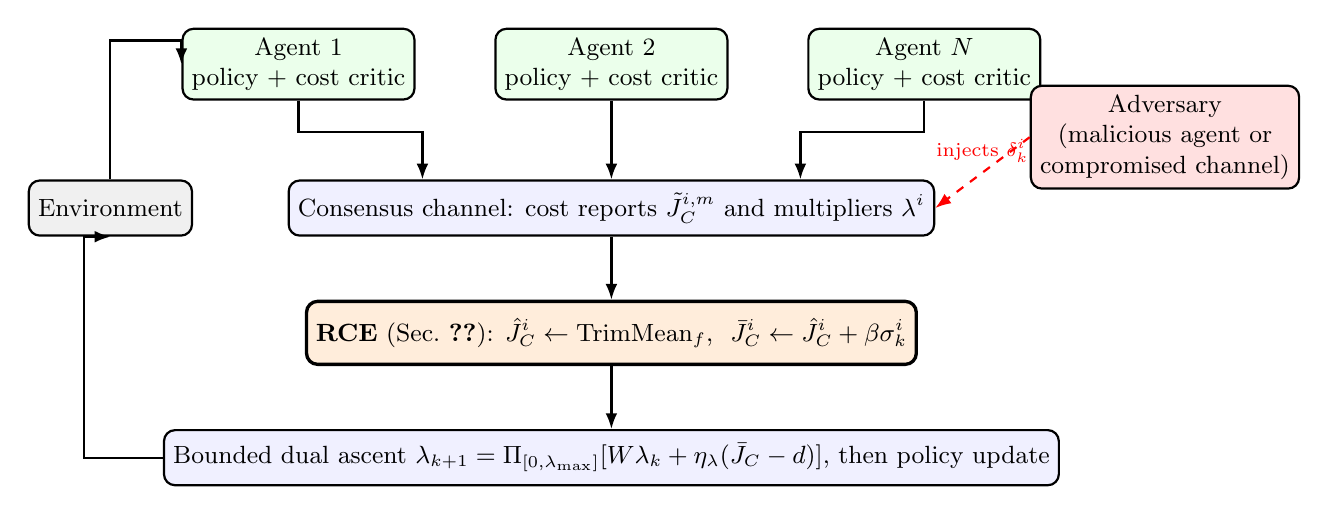
\begin{tikzpicture}[
  node distance=7mm and 10mm,
  box/.style={draw, rounded corners, thick, minimum height=7mm, align=center, font=\small, fill=blue!6},
  agent/.style={draw, rounded corners, thick, minimum height=7mm, minimum width=24mm, align=center, font=\small, fill=green!8},
  adv/.style={draw, rounded corners, thick, minimum height=7mm, minimum width=26mm, align=center, font=\small, fill=red!12},
  prop/.style={draw, rounded corners, very thick, minimum height=8mm, align=center, font=\small, fill=orange!14},
  arr/.style={-{Latex[length=2mm]}, thick}
]
\node[agent] (a1) {Agent 1\\policy $+$ cost critic};
\node[agent, right=of a1] (a2) {Agent 2\\policy $+$ cost critic};
\node[agent, right=of a2] (a3) {Agent $N$\\policy $+$ cost critic};
\node[box, below=10mm of a2, minimum width=76mm] (channel) {Consensus channel: cost reports $\tilde J^{i,m}_C$ and multipliers $\lambda^i$};
\node[adv, right=12mm of channel.east, yshift=9mm] (adv) {Adversary\\(malicious agent or\\compromised channel)};
\node[prop, below=8mm of channel, minimum width=76mm] (robust) {\textbf{RCE} (Sec.~\ref{sec:defense}): $\hat J^i_C \gets \mathrm{TrimMean}_f$, \ $\bar J^i_C \gets \hat J^i_C + \beta\sigma^i_k$};
\node[box, below=8mm of robust, minimum width=76mm] (update) {Bounded dual ascent $\lambda_{k+1}=\Pi_{[0,\lambda_{\max}]}[W\lambda_k+\eta_\lambda(\bar J_C-d)]$, then policy update};
\node[box, left=12mm of channel.west, fill=gray!12] (env) {Environment};

\draw[arr] (a1.south) -- ++(0,-4mm) -| ([xshift=-24mm]channel.north);
\draw[arr] (a2) -- (channel);
\draw[arr] (a3.south) -- ++(0,-4mm) -| ([xshift=24mm]channel.north);
\draw[arr, red, dashed, thick] (adv.west) -- node[above, font=\scriptsize, red] {injects $\delta^i_k$} (channel.east);
\draw[arr] (channel) -- (robust);
\draw[arr] (robust) -- (update);
\draw[arr] (update.west) -- ++(-10mm,0) |- (env.south);
\draw[arr] (env.north) |- ([yshift=3mm]a1.west) -- (a1.west);
\end{tikzpicture}}
\caption{System architecture. Cost estimates and multipliers are exchanged over a consensus channel before reaching constraint enforcement. An adversary at the channel or at a malicious agent injects $\delta^i_k$ (red). RCE sits between the channel and the dual update, and is the only component that distinguishes trustworthy from untrustworthy reports. Without it, corruption reaches the dual variable unfiltered and spreads across the network by Proposition~\ref{cor:spread}.}
\label{fig:architecture}
\end{figure}


\textbf{Configurations.} \texttt{ManyAgent Ant} with $N=6$ agents and cost limit $d=25$ per agent; \texttt{HalfCheetah} $2\times3$ with $N=2$; Safety-Gymnasium multi-agent navigation. Sources per constraint: $M=7$ in the primary setting, comprising the agent's own critic, four peer critics, and two replicated monitors. The $N=2$ setting uses $M=5$, obtained from two peer critics and three ensemble replicas, which is the configuration that demonstrates $M$ can exceed $N$.

\textbf{Hyperparameters.} PPO clip $0.2$, GAE $\lambda_{\mathrm{GAE}}=0.95$, discount $\gamma=0.99$, policy and critic learning rates $3\times10^{-4}$, dual step $\eta_\lambda = 0.035$, multiplier cap $\lambda_{\max}=25$, trim parameter $f$ matched to the assumed adversary count, margin $\beta=1.5$ unless swept, $10^7$ environment steps, 5 seeds. Baselines use the hyperparameters published with \citet{gu2023macpo}; RCE inherits them unchanged so that differences are attributable to the estimator rather than to tuning. Baselines are re-tuned under attack as a robustness check, since tuning benign and then attacking would confound the comparison.

\textbf{Attack implementation.} Corruption is applied to the return-scale residual $\tilde g^i_k = g^i_k + \delta^i_k$ after critic evaluation and before consensus, which is the point corresponding to a compromised channel. The adaptive variant sets $\delta^i_k = -\min(B,\; \kappa\,\max(0, \hat J^i_C - d^i + \nu))$, holding the reported residual just below the budget by a margin $\nu$ and thereby maximizing stealth subject to the budget.

\textbf{Compute.} Estimated $4$ GPU-days on a single A100-class device for the full grid of $3$ environments $\times$ $5$ methods $\times$ $4$ attack strengths $\times$ $5$ seeds, with the breakdown and $\beta$ sweeps adding approximately $1$ GPU-day.

\end{document}
